\documentclass{acm_proc_article-sp}
\usepackage{graphicx}
\usepackage{amsmath}
\def\url#1{{\tt#1}}

\begin{document}

\title{Advanced forensic Ext4 inode carving}

\numberofauthors{3} 
\author{
\alignauthor Jakub Marou\v sek \\
	\affaddr{Univerza v Ljubljani}\\
    \affaddr{Fakulteta za ra\v cunalništvo in informatiko}\\
    \affaddr{1000, Ljubljana}\\
    \email{jakub.marousek@gmail.com}%
\alignauthor Jan Ivanjko \\
	\affaddr{Univerza v Ljubljani}\\
    \affaddr{Fakulteta za ra\v cunalništvo in informatiko}\\
    \affaddr{1000, Ljubljana}\\
	\email{ji4988@student.uni-lj.si}%
\alignauthor Jernej Katanec \\
	\affaddr{Univerza v Ljubljani}\\
    \affaddr{Fakulteta za ra\v cunalništvo in informatiko}\\
    \affaddr{1000, Ljubljana}\\
	\email{jk6071@student.uni-lj.si}%
}

\maketitle
\begin{abstract}
Many widely-used filesystems (NTFS, FAT, Ext3) are well-researched in terms of digital forensics and data recovery, but this does not apply to Ext4, a successor in the family of Ext filesystems. Due to some new functionalities of Ext4 and compatibility breaking, a novel approach for file carving had to developed. The advantages of this approach include its ability to restore files even in the case of a corrupted superblock. This article gives a summary of the original paper and its outcomes, also with an introduction to Ext4 filesystem and Ext family included.
\end{abstract}

\section{Introduction}

In the present, Ext4 is a widely-used filesystem, especially on Linux-based operating systems and Android phones \cite{afeic}. The filesystem, released in 2008, has its origins in Ext2 and Ext3 filesystems. While many of their principles and structures were preserved (it is possible to upgrade from Ext2 or Ext3 in-place by setting new attributes), the changes are not just evolutionary. The way of storing and locating data blocks has changed, especially with the introduction of {\it extents}. From the forensical point of view, it was necessary to come up with new processes of recovering data.

This article provides a summary of the paper \cite{afeic}. But since the method is not easily understandable without wider information about Ext4 way of working, we include here a description of the filesystem. Furthermore, a description of Ext2 and Ext3 must be also attached, as Ext4 is closely tied to them and succeeds their functions.

Our work is organized in a following way: Section 1 is this introduction; Section 2 provides the description of the filesystems; Section 3 is the summary of the paper; in Section 4 results of the evaluation are described; and Section 5 is the conclusion.

\section{Introduction to Ext filesystem family}

The Ext4 filesystem is the next generation in the family of Ext filesystems, used typically in Linux environments. In the very beginning, the Linux kernel used Minix filesystem, due to the fact that Linux itself originated from Minix. This filesystem, however, contained serious limitations, the maximum file name size and the maximum filesystem size as the most severe examples. A group of kernel developers, with Theodore Ts'o being the most prominent one, introduced a couple of new filesystems \cite{ext2design}.

The first new filesystem, Ext (``extended filesystem'', released in 1992) removed the Minix limitations, but some of the previous problems remained -- for example, free blocks were monitored over a linked list, which harmed performance. As a quick response, Ext2 (``second extended filesystem'', 1993) was released. While the code of Ext2 originated in that of Ext, it brought many notable improvements.

\subsection{The Ext2 filesystem}

The filesystem supports standard Unix file types: regular files, directories, device-special files and links. The maximum size of a file is 2 GB, the maximum size of the whole filesystem is 4 TB.
As the other Unix filesystems, it also uses inodes for storing file metadata. An {\it inode} is a structure containing a description of a file: file type, access rights, owners, timestamps, size, pointers to data blocks.

A directory is only a special kind of file, with a list of files and their corresponding inodes. A link can be either hard or symbolic. A hard link is basically a file pointing to the same inode as the original file, not distinguishable from the previous file. To remove a hard-linked file, all the references to the file must be removed. A symbolic link contains a text specifying a path to the file. Unlike the symlink, creating a hard link has limitations: it is possible to hard-link only a file from the same partition (due to the nature of the link) and hard-linking directories is not allowed (to prevent infinite subdirectory loops). A device-special file is only a pointer to the device driver.

While these features are common for all Unix filesystems, now we shall list some abilities specifical for Ext2. Using the file attributes, the kernel behavior of creating new files in a directory can be modified, specifically the new file user id and group id. The logical block sizes can be specified when the filesystem is created -- larger block sizes lead to efficient behavior, but also wastes more space.

The symbolic links of Ext2 can use more efficient way of storing the path inside the inode of the symlink. The overall status of the filesystem is saved in the superblock. During the mounting of the filesystem, if it is detected that it was not unmounted properly, the filesystem is automatically checked. After a certain number of mounts or when a certain time period has passed, the filesystem checking is enforced.

It is also possible to create {\it immutable} files, which either cannot be written into or deleted, or they can be opened for writing, but the text is appended to the end of the file.

\begin{figure}
\centering
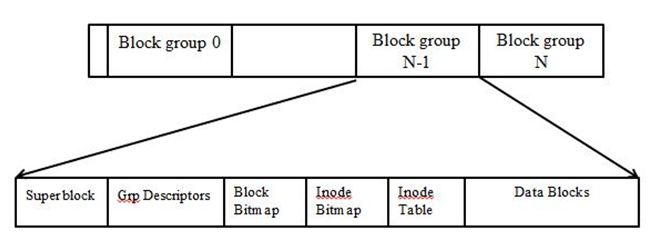
\includegraphics[width=0.48\textwidth]{images/ext2structure.jpg}
	\caption{The structure of an Ext2 filesystem \cite{ext2structure}}
\end{figure}

{\bf The filesystem structure} is as follows. There is a boot sector in the beginning of the space, which is designated for bootloaders code. The rest of the drive is split into {\it block groups}. Each block groups contains inodes (in an inode table) and data blocks. An inode bitmap and a block bitmap marks which inode/block is used and which is not. 

The superblock and group descriptors contain information which are crucial for the filesystem functioning, and thus they are put in the beginning of each group as a backup. The superblock contains the basic information about the structures, like logical block sizes, the number of blocks and inodes, positions of data blocks and so on. An array of group descriptors contains pointers to the inode table and the block table for every present group.

As the main optimization, Ext2 performs block readahead, that means, reads more continguous blocks at once. Block groups try to keep together inodes and blocks of a file, which reduces disk seeks. Also when a file is being written, Ext2 preallocates up to 8 blocks.

\subsection{The Ext3 filesystem}

After the initial period of bugs elimination, the Ext2 filesystem has become a safe, stable choice for a Linux-based operating system. One of the main drawbacks of using Ext2 is the lack of jounrnaling, which slows down the filesystem check and makes files prone to corruption.

First suggestions for the journaling of ext filesystem family were put down by Stephen C.\ Tweedie \cite{extjournal}. He identifies several aspects of filesystem reliability and puts forward {\it preservation} (``stable'' data on the disk should never be damaged), {\it predictability} (the failure modes of the filesystem should be predictable and deterministic) and {\it atomicity} (every operation is either fully performed or fully undone). The Ext2 provided only the preservation aspect, whilst the failure states (could occur because of an unexpected reboot, for example) were not properly defined and might have prevented the operations from fully performing.

The Tweedie's article \cite{extjournal} compares approaches of reaching the desired aspects. The easiest way is to wait for a disk write to complete before the next one is submitted, which breaks the performance. Another idea lies in preserving multiple write buffers, ordering them accordingly and write these separately. However, one can easily get into a situation when the buffer dependendence is cyclic (moving a file from directory $A$ to directory $B$ and, in the same time, moving another file from $B$ to $A$). While there exists a mechanism to solve it, all the presented approaches require the disk to be completely rescanned for errors in case of a system failure. (Recall that filesystem check slowness was one of main objections against Ext2.)

Instead, the author proposes to use {\it journaling}. To ensure operations to be atomic, a batch of data is written on the disk, but is not effective until a special {\it commit} block does not conclude the operation. Thus, a failure during performing the write can result only in two possibilities: either the commit block has been written on the disk, which means the transaction is complete, or it has not been written, in which case the transaction as a whole is undone. More practically: there is a dedicated place on the disk, called a {\it journal}, working as a cycling buffer. A transaction starts with a description block, continues with all the blocks that the transaction is modifying, and end with a commit block. Only after all these blocks have been successfully written to the journal, the ``real'' blocks modification is done. If a failure of the system occurs, the recovery program goes through the journal and performs all transactions which contain the commit block. If the block is not present, the transaction is discarded.

\begin{figure}
\centering
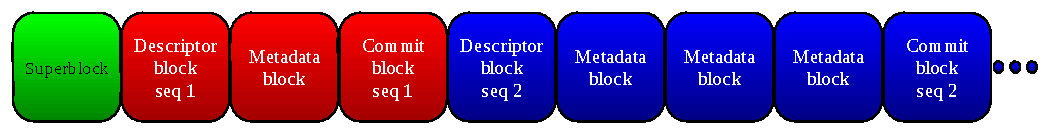
\includegraphics[width=0.48\textwidth]{images/journal.pdf}
	\caption{The structure of Ext3 journal \cite{takingadvantage}}
\end{figure}

The Ext3 filesystem, released in 2001, i offers three different modes of journaling: \cite{takingadvantage}

\begin{itemize}
	\item {\it Journal} -- All data and matadata are logged. This approach minimizes the chance of losing data, but has the laregst performance penalty.
	\item {\it Ordered} -- Only metadata are logged, but file data are flushed on the disk before the change of metadata occurs, keeping the journal synchronized with data writes. This is the default mode.
	\item {\it Write back} -- Only metadata are logged, file data are flushed whenever possible. This mode is the fastest, but also the most dangerous.
\end{itemize}

Notice that journaling cannot be turned off. Compared to Ext2, this is the only different feature. Thanks to this, it is possible to convert an Ext2 partition to Ext3 with spawning a single command.
For the period of Ext3 development, a principle of both backward and forward compatibility with Ext2 was closely followed by its authors. Therefore, an Ext3 partition can be mounted with Ext2 driver and works the same with the exception of journaling. Turning off a journal causes an Ext3 partition to become Ext2 and vice versa.

\subsection{The Ext4 filesystem}

Although Ext3 was a step forward, it still lacked some state-of-the-art features, which could be found in other Unix filesystems. Between 2003 and 2006, numberous patches for the Ext3 were proposed to be added to the Linux kernel, but they were not accepted because the Linux community was afraid of stability of their mostly-used-filesystem at that time. As a result, Theodore Ts'o introducted plans for creating a successor of Ext3, which would partially break the forward compatibility, but still allowed an easy update from the older versions \cite{newext4}. In 2008, the code was marked as stable.

A large amount work was done in terms of scalability. The maximum size of the filesystem was raised to 1 EB, the maximum size of a file is raised to 2 TB. The maximum number of files is increased too.

A compatibility-breaking change of file block locations is brought up. Instead of storing a list of data blocks (which is advantageous for small files but unpractical for large ones), {\it extents} are introduced. An extent is a range of data blocks, where all blocks in the range belong to the file. Four extents can be directly stored in the inode of the file. For large and fragmented files, a tree of pointers is maintained, with extents being in the leaves.

\begin{figure}
\centering
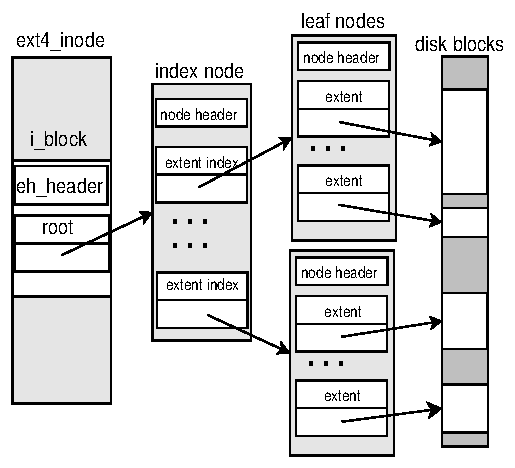
\includegraphics[width=0.48\textwidth]{images/extents.pdf}
	\caption{Extent tree layout \cite{newext4}}
\end{figure}

The transactions in the journal are checksummed in the commit block, making two consequences: the recovery is more reliable as the corrupted transaction blocks are detected and the transaction cancelled; also now the commit block can be written in the same time as the other blocks, which significantly improves the performance.

Contrary to Ext4, persistent pre-allocation of file size is possible. The checking of the filesystem is 2 to 20 times 2 to 20 times faster, as the unallocated inodes are marked and are skipped during the rest of the procedure. Instead of allocating one block at a time, the allocation is {\it delayed} in Ext4, meaning it is postponed in time and performed when the file is flushed. There is also a possibility of online defragmentation. Since the size of an inode is larger, nanosecond resolution timestamps are supported and the problem of year 2038 is deferred for 272 years.

Similarly as in the case of Ext2 and Ext3, migrating to Ext4 is just a matter of turning on the new features. The legacy system of individual block mapping is preserved, but all new files will use extents. Downgrading from Ext4 to Ext3 by turning off the features is straightforward when extents are not used -- otherwise, temporary copy of the files is needed.

\subsection{Comparison of Ext4 and other Unix filesystems}

It is worth noting that Theodore Ts'o considered Ext4 not to be a major advance and still using old technology. In the light of his words, I found potentially interesting to list other popular Unix filesystems and compare their functions.

{\it Btrfs} \cite{btrfs} is a filesystem brought to life by Oracle. The development began in 2007 and the software was proclaimed to be stable in 2014. The name comes from the B-tree as this is the main structure used within the filesystem. Notable features of Btrfs are copy-on-write (a copied and unmodified file references to the ``old data''), snapshots, CRC checksums of data, RAID or configurable compression. In order to prolong the lifespan, SSD drivers are handled specifically. In-place conversion from Ext2/3/4 and ReiserFS is present.

{\it ReiserFS} was created by company Namesys with Hans Reiser as the chief developer. When the first version was released in 2001, it brought attention because of features which had been unavailable, like journaling, online filesystem resizing, packing files in a single disk block or B-tree usage. Although ReiserFS was popular in the past, it was overtaken by other filesystems since then. The main reason may be the slow pace of development, especially after Hans Reiser has been imprisoned and convicted of murder.

{\it ZFS} \cite{zfs} was developed by Oracle, but after the end of support the project was handled to the open-source community \cite{openzfs}. It supports journaling, read-only snaphots of the files state, RAID or checksums of files. On Ubuntu, ZFS has been chosen as the default filesystem for containers.

\section{File carving in Ext4}

File carving, or sometimes just "carving" is the process of extracting data collection from a larger data set. Digital investigation often include data carving techniques when unallocated filesystem space is analysed to extract files. These files are carved from the unallocated space using file type-specific header and footer values\cite{merola2008data}.

File carving is not the same as file recovery. File recovery techniques rely on the filesystem information that remains after the deletion of a file to recover those files. On the other hand file carving techniques are used to restore as much data or data fragments as possible, when the filesystem is corrupted or deleted. Carving or raw data recovery process does not rely on the filesystem structures. It searches block by block for data matching the specific file type header and footer values\cite{beek2011introduction}. 

In digital forensics carving is especially useful in criminal cases, becouse it can recover evidence. As long as data on a disk is not overwritten or wiped, it can be restored using file carving techniques. Sometimes even data from formatted drives can be restored if the conditions are right. The most common general techniques to carve files are\cite{hadi2016reviewing}:

\begin{itemize}
\item \textbf{File Structure Based carving}
This technique uses identifier string, header, footer and size information to assume internal layout of a file. Header is a unique identifier, its value identifies the type of a file. Its existence means we can identify the beginning of a file, while the existence of a footer shows the tail of a file.
The blocks between the header and the footer represent the targeted file. In some cases file format has no footer, therefore a maximum file size is used in the carving program.
\item \textbf{Content based carving}
Carving based on content structure (MBOX, HTML, XML) or linguistic analysis of the file's content. A semantic carver might conclude that some blocks of German in a middle of a long HTML file written in English is a fragment left from a previous allocated file, and not from the English HTML file. Similarly for other content characteristics like, character count, information entropy, white and black listing of data.
\end{itemize}
Carving can be classified as basic and advanced, with basic it is assumed that:
\begin{itemize} 
\item the beginning of file is not overwritten
\item the file is not fragmented
\item the file is not compressed
\end{itemize}
Advanced carving relies on internal file's structure and occurs even to fragmented files, where fragments can be:
\begin{itemize} 
\item not sequential
\item out of order
\item missing
\end{itemize}
Since basic carving does not consider the file's content the  attention has shifted to  advanced  carving methods. Header and footer are not enough to carve files because the file's content is not checked nor is sector within header/footer examined. Deeper knowledge of internal file's structure results in less false positives. 

Authors of the paper present an advanced method that uses patteren-based file carving . It searches for metadata structures of inodes to recover their content data. This approach avoids reading the superblock and group descriptor table since its goal is to recover files from reformatted or corrupted Ext4 filesystems. The presented method can be divided into five phases\cite{dewald2017afeic}:
\begin{enumerate}
\item \textbf{Initialization}

The point of initialization  is to gather Ext4 parameters, they can be estimated from the filesystem size. The following parameters are of relevance:
\begin{itemize} 
\item Offset
\item filesystem size
\item Block size
\item Inode size
\item Inode ratio
\item Flex group size
\item 64 bit mode
\item Sparce superblock
\item Number of blocks per block group
\item Numbers of blocks and block groups in the filesystem
\item Number of inodes per block group
\item Space for growing group descriptor table
\end{itemize}
\item \textbf{Inode carving}

Not every 128 byte permutation forms a valid inode. For an inode to be correct, some of the values must be in certain relations. This fact is used while searching for potential inode candidates in a byte wise manner. The most significant 4 bits in the 2 byte structure of inode indicate its file type.

Search patterns can also be based on timestamps, such as time interval or its inner consistency. Creation date, modification date, deletion date timestamp consistency can be verified if the following conditions are true:
\begin{itemize}
\item Modification date\textless creation date
\item Deletion date=0 and (deletion date\textgreater modification date and deletion date\textgreater creation date
\item Modification, creation time and delete time must be valid
\end{itemize}
Extent header field must contain the statisticaly defined magic number 0xf30a. Other inode attributes can be used for search patterns. All found addresses of potential inodes are sorted by file type (regular files and directories) and used for recovery.
\item \textbf{Directory tree}

This phase tries to identify potential directory inodes. Directory entries are searched linearly where directories not strating with '.' or '..' are discarded. The file name and inode number are saved along with its parent inode number, therefore a logical tree forming the complete file path can be deducted.

The module must map physical inode addresses to inode numbers. The beggining of the inode table can be computed by equation:

\[s=(bg_a * n_{BG} +o_s + o_i +o_r)*b  \]
The mapping of an address to its inode number is computed by:

\[o_s=min \{1024, 1+ \left\lceil \frac{d*n_g+1024}{b} \right\rceil \} \]
\[ o_s=2*n_f\]
\begin{equation}
  X=
  \begin{cases}
    0, & \text{if}\ b=1024 \\
    1, & \text{otherwise}
  \end{cases}
\end{equation}
\[bg_a=\left\lfloor \frac{a}{b*n_{BG}} \right\rfloor \]

\[f(a)=(\frac{a-s}{i} +n_{i,BG} *bg_a +1) \]

where:
\begin{itemize}
\item b block size

\item $bg_a$ is block group of address a

\item $n_{BG}$ is number of inodes per block group

\item $o_s$ combined size of superblock, the group descriptor table and growth space

\item $o_i$=2*$n_f$, offset where $n_f$ is flex group size

\item $o_r$ first 1024 bytes of the filesystem are reserved independently of block size. This offset is in case the block size is 1024 and the reserved space takes whole block, shifting all addresses by one block 

\item i size of inode 
\end{itemize}

The mapping from physical addresses to inode numbers can be done using these formulas. By using information from directory trees, file names can be associated to inodes. In case of a irreparable directory, its children's file paths can not be reconstructed therefore their content is saved in files named after their inode address. All recovered files are named after their inode address and saved into a flat hierarchy.



\item \textbf{Regular files}

Having reconstructed file path or not the content of a regular file is now recovered. Ext4 filesystem stores file content scattered across the volume in a way managed by the extents. Since the filesystem journal can contain copies of the existing inodes, duplicates with different physical addresses can be found. In order for two inodes to be the same, the file size and the extent structures are compared, due to the lack of inode numbers.
\item \textbf{Files without content}

This is another optional phase and builds on the results of the directory tree and content data phase. The content of files found in the directory tree phase but not in the inode carving phase, cannot be recovered, but their filepath can. Therefore files are created empty with their original filename and file path.
\end{enumerate}

\section{Evaluation of the method}

In the previous sections, an approach for reconstructing inodes was introduced. It is based on search patterns of different inode attributes. All inodes that match the patterns are considered potential inodes. Using their extent tree, the file content can be reconstructed. In this section, we present an evaluation of the quality of each search pattern and also the completeness and correctness of presented tool. It was firstly introduced in the 2017 paper by A. Dewald and S. Seufert \cite{afeic}.

\subsection{Dataset}

They have built a dataset with different hard disk images to evaluate their approach and Sleuthkit implementation of the tool. They have used different filesystem sizes to cover different configurations that can occur when formatting disks of different sizes with default values. 
Further, they have built test cases where they deleted specific files or changed filesystem parameters that might influence the success of the approach.
They distinguished two for images where they have deleted files:
\begin{itemize}
\item files that have been deleted directly
\item files that have been deleted by moving to the trash first.
\end{itemize}
They also made a case where they deleted all files and copied new ones on the filesystem to check if the former files can be recovered.
Further, they compared Ext4 filesystems with enabled and
disabled journal and deleted files. To create a more realistic
example image, they created one that contains an entire Ubuntu
Linux installation with various files that have been moved, deleted
and modified and also containing symbolic links, device files and
other non-regular file types to cover a broad spectrum.
At the end, they created images where they overformatted the existing Ext4 with NTFS or again Ext4. For each of those cases, they compared standard and quick formatting. The dataset contained mostly small images.

\subsection{Search patterns and selectivity}

In the paper, they checked, how well the different patterns perform. 
To test this, they choose the image with installed Ubuntu and various cases. They used the Sleuthkit tool fsstat to provide a ground truth about the number of reserved inodes.
Considering the first 10 inodes to be reserved, there remained 201.269 files, of which they checked how many are regular files and directories.

Each pattern was tested on each physical address and can accept or decline this address as potential inode. Accepted addresses that lie within an area of an inode table at a valid offset and can be reconstructed successfully are listed as hits in the table. This is the total number of files in the filesystem. Table misses are structures that might be a valid inode, but reside outside an inode table. Those could be false positives, but could also be copies of inodes for example in the filesystem journal. Similarly, address misses are potential inode addresses that do not lie at a 128 byte inode boundary.

Misses do not necessarily mean false positives, so they are not rejected at the first place. The number of accepted addresses for the pattern is the sum of t-misses and a-misses, while the selectivity of each pattern is the number compared to the total number of possible addresses.

Table 1 shows the number of identified potential inodes for each pattern. 'k' stands for thousand, 'M' for million and 'G' for billion, while t-miss are table misses, a-miss are address misses. The selectivity is hits compared to all misses.

\begin{table}
\centering
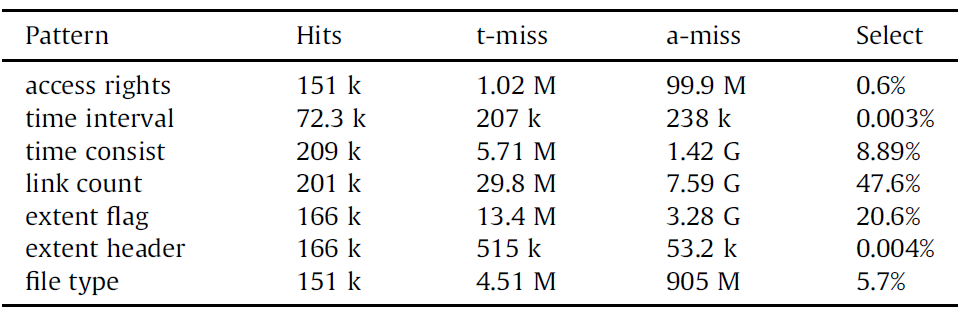
\includegraphics[width=0.48\textwidth]{images/selectivity.png}
	\caption{Search pattern selectivity}
\end{table}


In the following sections, we discuss the results for each pattern in detail.

\subsubsection{Access rights}

While there is no illegal combination for access rights, a search pattern can be defined to search for files with specific rights or to cover the most common access right combinations. In the configuration file of the proposed tool, the pattern can be adjusted. For the experiment, they choose the most common combinations of access rights in Linux systems. They are shown in table 2
This pattern accepted only 142.855 valid inodes out of 201.269.  However, this contained almost all regular files and folders.

\begin{table}
\centering
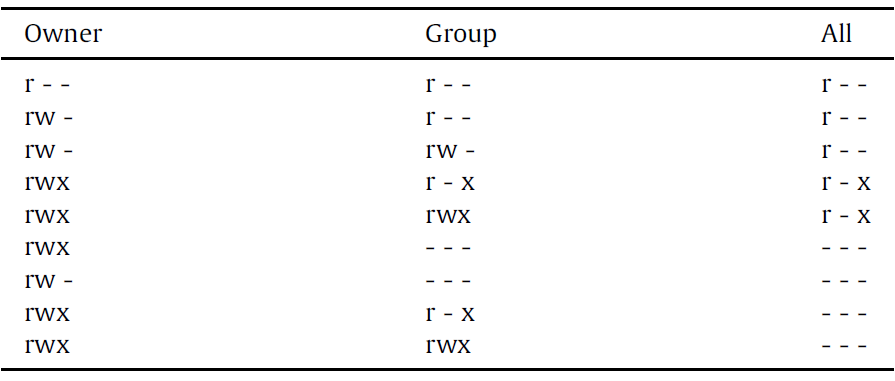
\includegraphics[width=0.48\textwidth]{images/rights.png}
	\caption{Access rights patterns chosen for the experiment}
\end{table}

\subsubsection{Timestamps}

The timestamp pattern consists of two parts: firstly, they validated the inner consistency of the different timestamps, and in the second part, the investigator might configure a relevant timeframe for his case. For this experiment they choose the timeframe from 2015-01-01 00:00:00 GMT to 2016-01-01 00:00:00 GMT, in which the system was set up and all actions have been performed. Amongst the potential inodes have been 7.140 false positives, so that the number of hits was reduced to 65.170.

With respect to only the inner consistency, they obtained 209.481 hits, 5.708.816 t-misses and 1.416.653.929 a-misses. 8.213 of the hits have been identified as false positives, however, all other valid 201.264 have been found.

\subsubsection{Number of hard links}

In the paper, they have checked whether the internal number of hard link counter of a potential inode is larger then 0. All 201.269 potential inodes were accepted by this, beside special inodes 7 and 8, which are counted as false positives.

\subsubsection{Extent flag and header}

Researchers evaluated the pattern for the extent flag and extent headers separately. The selectivity of the second header is very high, because of the 2 byte magic number. Its pattern is the only pattern, that produces far more table misses that address misses. This pattern also matches various content data blocks. However, all regular files and folder have been accepted by this pattern, along with 8.074 false positives. 
Also, inodes of deleted files are accepted by this pattern too. 

\subsubsection{File type}

The authors of the paper were restricted only to regular files and folders, so they adjusted the file type pattern accordingly. Besides 8.068 false positives, this pattern matches on all 142.919 inodes they searched for.

\subsubsection{Pattern combination}

In this experiment, 3 most restrictive patterns were the extent headers, timestamp intervals and access rights. Last two include some semantic filtering, so researchers did not include them in the next experiments to verify correctness of the tool.

\subsubsection{Completeness and correctness}

To evaluate completeness and correctness of the tool, both operation modes of the tool were testet and compared. Correct recovery was checked with MD5 and SHA256 hashes. In the contentdata mode, the files need to be reconstructed with the correct values, while in the metadata mode also the file name and path have to be correct, in order to consider correct recovery.

The authors of the research evaluated two images of different categories. First, they evaluated the tool on the real case images to verify correctness and completeness by comparing the results of the tool the known ground truth. Second, they wanted to evaluate, whether they can recover files from filesystem that have been overformatted.

\subsection{Real world cases}

Researchers presented some real world cases. In their first case, the metadata mode reconstructed empty files with the correct file names and paths for all non-regular files and all files and folders that have been
placed correctly. On the other hand, in the contentdata mode, folders were not reconstructed, but all the placed files had been recovered correctly.

They created one image by sending all files on the image to trash. The trash contained all the original files, as well as metadata files that documented the original paths and times for deletion, which all had been recovered by the tool.

In the next step, they emptied that trash. In metadata mode, the tool only recovered the empty root and trash folder. But in the contentdata mode, all files were reconstructed correctly, just without original file names. 

They went further and they deleted all files from images with sending them to trash and emptying it. After that they copied new files to the resulting new images. The metadata mode recovered all newly written files correctly from all images. The contentdata mode was also able to recover one file form the original filesystem, whose file content had not been overwritten by new files. Its inode resided in the old journal.


\subsection{Overformatted filesystems}

In this section, the evaluation, if it is possible to reconstruct files from Ext4 that have been overformatted in different ways, is given. The researchers evaluated this on small image, which provided an upper boundary of what files can be reconstructed.

They overformatted the original file with Ext4 and NTFS filesystems in full formatting mode. In those cases, the blocks had been zeroed and they were not able to recover any files. Ext4 as well as NTFS provide an option for so called fast formatting, where no blocks are zeroed while formatting and only newly used blocks are overwritten.

The image \texttt{small\_fastExt4.img} 
 had been created by using the same default parameters when overformatting the volume as used for the original formatting. The tool recovered all but 3 of the original files and all but 2 folders in the metadata mode, while in the contentdata mode it additionally recovered the journal from inode 8 as a file.

In \texttt{small\_fastdiffExt4.img} non-default parameters had been used 
 for formatting. None of the original inode table resided in areas that had not been overwritten and the metadata mode was not able to recover files. The journal had not been overwritten, so that in the content data mode, the tool was able to recover 125 files, of which 52 were totally unmodified, but the others had been partly overwritten.

In the image 
\texttt{small\_fastNTFS.img}
, the structures that had been created for the NTFS filesystem, did not overwrite the area of the original inode tables and both operation modes were able to recover all the original files, of which only some had modified content and some blocks had been used by the new filesystem.

Table 3 lists the number of found inodes and files from the fast overformatted filesystems and compared results from both modes of the tool.

\begin{table}
\centering
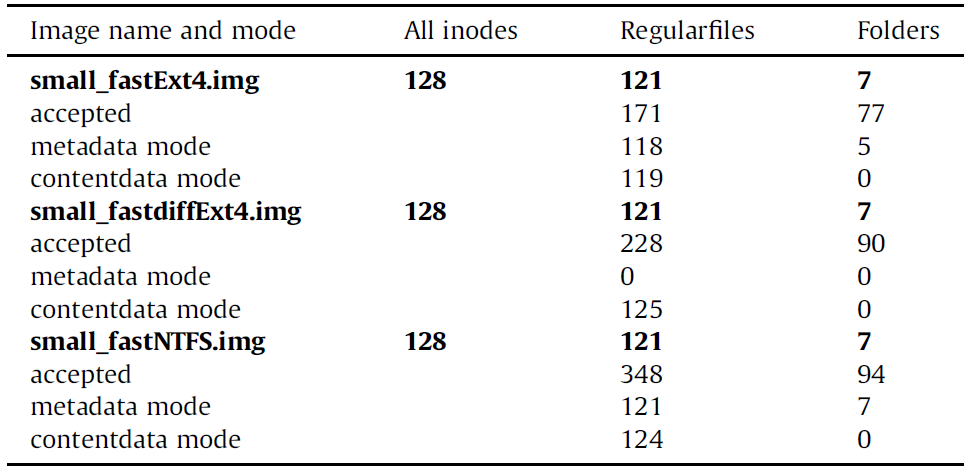
\includegraphics[width=0.48\textwidth]{images/number.png}
	\caption{Number of found inodes after selection of the overformatted dataset}
\end{table}

\subsection{Runtime performance}

Both implemented methods show similar speed, while the contentdata mode is slightly faster. The runtime is linear in dependence from the image size. Both approaches take about 30s per GB image size.

\section{Conclusions}

In this article, we have introduced the readers to the structure and functioning of Ext2, Ext3 and Ext4 filesystems. For Ext4, we have presented a novel approach of data recovery, which is able to restore data even in case of a corrupted superblock \cite{afeic}. The solution was proved to be successful in many situations and was adapted for Sleuthkit framework.

%In future work, the authors want to add backward compatibility, so even Ext4 filesystems upgraded from Ext3 would be also supported. This is not possible now, as only extents are considered, not (in)direct pointers, which initially remain in a converted Ext4 filesystem.

\bibliographystyle{abbrv}
\bibliography{paper}

\balancecolumns
\end{document}
